\documentclass[12pt]{article}
\usepackage[a4paper, total={7.5in, 11in}]{geometry}
%\usepackage{array}
\usepackage{graphicx, subfig, wrapfig, fancyhdr, lastpage, multicol ,color}
\newcommand\headerMe[2]{\noindent{}#1\hfill#2}
\usepackage[mathscr]{euscript}
\usepackage{tabularray}

\setlength{\columnseprule}{1pt}
\def\columnseprulecolor{\color{blue}}


\pagestyle{fancy}
\fancyhf{}

\cfoot{ \vspace{-0.8cm}\em{Page \thepage \hspace{1pt} / \pageref{LastPage}}}
\begin{document}

\headerMe{Royaume du Maroc}{année scolaire \emph{2024-2025}}\\
\headerMe{Ministère de l'Éducation nationale, }{  Professeur :\emph{Zakaria Haouzan}}\\
\headerMe{du Préscolaire et des Sports}{Établissement : \emph{Lycée SKHOR qualifiant}}\\

\begin{center}
Devoir Surveillé  N°1 - semestre 02 \\
    2ème année baccalauréat Sciences Mathématiques\\
Durée 2h30
\\
    \vspace{.2cm}
\hrulefill
\Large{Chimie 7pts/42min}
\hrulefill\\

	\emph{Toutes les solutions sont prises à 25°c, et $K_e=10^{-14}$. }
\end{center}
%end Headerss------------------------
%__________________Chimie ______________________-
%%%%%%%+_+_+_+_+_+_+_+_+_Partie1

 \section*{Partie 1 :Amines et composés apparentés \dotfill(7pts) }

 \emph{Les amines sont des composés organiques qui se caractérisent par des solutions
aqueuses basique. On s’intéresse à l’étude d’une solution aqueuse d’une amine A de
formule $C_2H_5NH_2.$ }

On prépare une solution S0 de cette amine de concentration $C_0=2.10^{-2} mol/L$ et de $pH_0=11,55$ à 25°c.

\begin{tblr}{c|[dashed]l}
	1  & {\textbf{1.1. }Ecrire l’équation de réaction de l’amine A avec l’eau, et dresser le tableau
	d’avancement\\pour un volume V.} \\
	0.5  & \textbf{1.2. }Calculer le taux d’avancement final de la réaction. Conclure.\\
	1  & \textbf{1.3. }Calculer la valeur de $pK_A$ du couple acide/base de l’amine A. \\
	1.5  & {\textbf{1.4. }On dilue la solution $S_0$, pour obtenir une solution $S_1$ de concentration
	$C_1=10^{-2} mol/L$ . \\En négligeant la dissolution de la base avec l’eau, montrer que le
	pH de la solution $S_1$ peut\\ s’écrire sous la forme : $pH = 7 + \frac{1}{2}.(pK_A + log(C_1)$.
Calculer $pH_1$. } \\
\end{tblr}

\textbf{2.} On prend $V_1=10mL$ de la solution $S_1$, et on procède au dosage avec une solution
aqueuse d’acide chlorhydrique $(H_3O^+_{(eq)} + Cl^-)$ de concentration $C_2=10^{-2} mol/L$.
L’évolution de la valeur de pH du mélange au cours du dosage, est représentée par la
courbe de la figure .

\begin{center}
  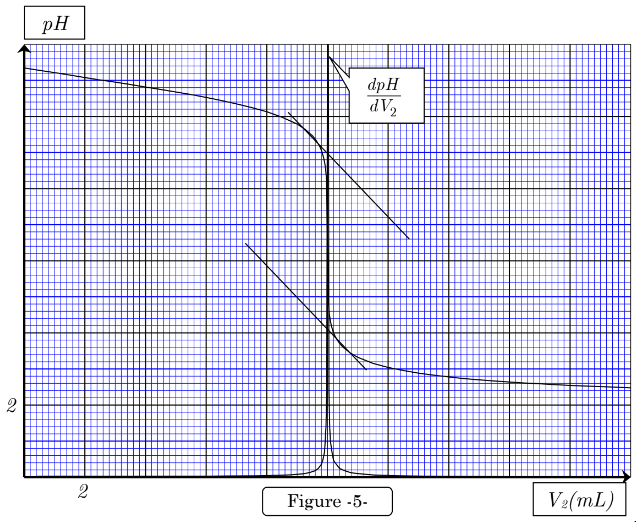
\includegraphics[width=0.6\textwidth]{./img/chimie00.png}
\end{center}


\begin{tblr}{c|[dashed]l}
	0.75  & {\textbf{2.1. }Ecrire l’équation de réaction du dosage, et calculer sa constante d’équilibre.
\\Que peut-on dire de la nature de cette réaction ? } \\
	0.75  & {\textbf{2.2. }Déterminer les coordonnées du point d’équivalence, puis vérifier la valeur de la
$C_1$. }\\
	1.5  & {\textbf{2.3. }Calculer les concentrations de l’amine A et de son acide conjugué lorsqu’on a
versé \\un volume $V_2=16ml$ de la solution titrante. En déduire le pourcentage de
chacun. } \\
\end{tblr}
%\hrulefill
%\Large{Physique 13pts/78min}
%\hrulefill\\
\begin{center}
    %\vspace{.60cm}
\hrulefill
\Large{Physique 13pts}
\hrulefill\\
    \emph{Les deux parties sont indépendantes}
\end{center}


\section*{Partie 1:Electricité (1) \dotfill(7pts) }

\begin{wrapfigure}[3]{r}{0.25\textwidth}
	\vspace{-1cm}
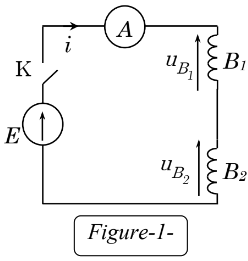
\includegraphics[width=0.9\linewidth]{./img/phys00.png} 
\end{wrapfigure}

On réalise le circuit électrique représenté dans
la figure-1- comportant :
\begin{itemize}
	\item Un générateur de force électromotrice E.
	\item Une bobine d’inductance $L_1$ et de résistance
interne $r_1$.
\item Une bobine d’inductance $L_2$ et de résistance
interne $r_2$.
\item Un ampèremètre et un interrupteur K.
On ferme K à t=0.
\end{itemize}

\begin{tblr}{c|[dashed]l}
	0.5  & {\textbf{1. }Montrer que l’équation différentielle vérifié par l’intensité du courant i(t)
	s’écrit \\sous la forme : $i + \tau.\frac{di}{dt} = \alpha$ \\
	Avec $\tau$ et $\alpha$ , des constantes dont on déterminera les expressions.
	}\\
	
	1 & {\textbf{2. }La solution de cette équation s’écrit sous la forme : $i(t) =A.e^{-\lambda.t} + B$. En
utilisant les \\conditions initiales et les caractéristiques du régime permanant,
trouver les expressions des \\constantes A et B.  } \\
	\end{tblr}

\textbf{II. }La courbe de la figure -2 montre les variations de l’intensité du courant
i(t), et la figure -3-, celles des tensions ${u_B}_1(t)$ et ${u_B}_2(t)$ aux bornes des bobines.

\begin{center}
  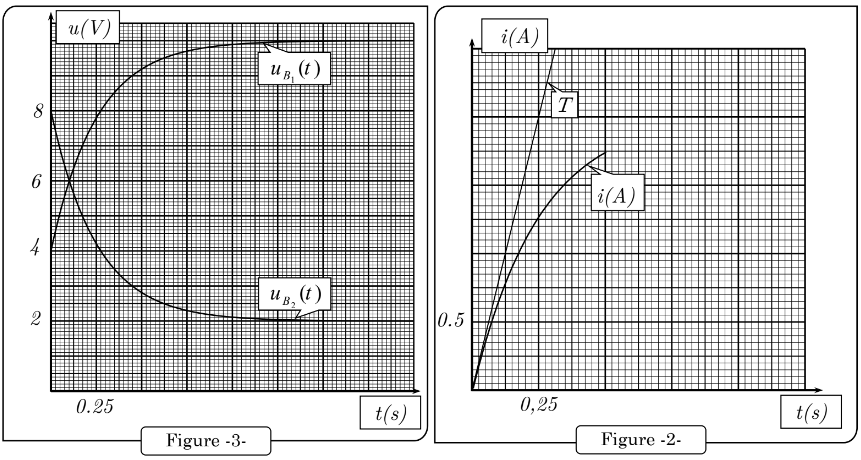
\includegraphics[width=0.7\textwidth]{./img/phys01.png}
\end{center}
\begin{tblr}{c|[dashed]l}
	0.5  & {\textbf{3. }Montrer que E=12V. }\\

	0.5 & {\textbf{4. }Trouver l’expression de $\frac{di}{dt}(t = 0)$, à $t=0$ en fonction de E, $L_1$, et $L_2$}.\\
	
	1 & {\textbf{5. }La droite T dans la figure-2, représente la tangente à la courbe i(t) à t=0.
	Trouver graphiquement \\la valeur $\frac{di}{dt}(t=0)$, et en déduire la valeur de $L_1+L_2$. }.\\

	0.75 & {\textbf{6. }Montrer que $u_{B1}(t = 0) = \frac{L_1}{L_1 + L_2}.E $ et $u_{B2}(t = 0) = \frac{L_2}{L_1 + L_2}.E $\\
	En utilisant les courbes de la figures -3, trouver les valeurs de $L_1$ et $L_2$.
	}.\\

	0.75 & {\textbf{7. }Montrer qu’en régime permanant, les tensions  $u_{B1}(\infty) = \frac{r_1}{r_1 + r_2}.E $ et $u_{B2}(\infty) = \frac{r_2}{r_1 + r_2}.E $  }.\\
	
	0.5 & {\textbf{8. }En régime permanant, l’ampèremètre affiche la valeur $2A$. Calculer les valeurs de $r_1$ et $r_2$. }.\\
	
	1.5 & {\textbf{9. }L’expression de la tensions $u{B_1}(t)$ s’écrit sous la forme : $u_{B_1} = C + D.e^{\frac{-t}{\tau}}$ \\Trouver les expressions des deux constante C et D. }.\\

\end{tblr}


\section*{Partie 2 : Electricité(2) \dotfill(6pts) }

\begin{wrapfigure}[3]{r}{0.25\textwidth}
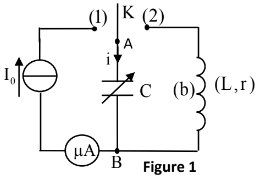
\includegraphics[width=0.9\linewidth]{./img/phys02.png} 
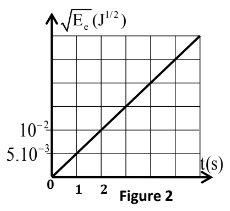
\includegraphics[width=0.9\linewidth]{./img/phys03.png} 
\end{wrapfigure}


Cet exercice vise l’étude de la charge d’un condensateur et sa décharge dans une bobine.

\textbf{I- Charge d’un condensateur et sa décharge dans une bobine : (3pts)}
On réalise le montage représenté sur le schéma de la figure 1. 

Ce montage comprend:
\begin{itemize}
	\item --un générateur idéal de courant.
	\item --un condensateur de capacité C variable, initialement non chargé.
	\item --une bobine(b) d’inductance $L =  8,6mH$ et de résistancer $r = 12\Omega$
	\item --un microampèremètre
	\item --un interrupteurK.
\end{itemize}

On ajuste la capacité du condensateur sur une valeur $C_0$. On place l’interrupteur K en position (1) à un instant de date
$t=0$ .Le microampèremètre indique $I_0 = 10\mu A$. Un système de saisie
informatique convenable permet d’avoir le graphe de la figure 2
représentant $\sqrt{E} = f(t)$ avec $E_e$ étant l’énergie électrique emmagasinée dans le condensateur à un instant t.

\begin{tblr}{c|[dashed]l}
0.25  & {\textbf{I.1. }Donner l’expression de l’énergie emmagasinée dans le condensateur \\en fonction de sa charge q et de sa capacité $C_0$} \\

0.75  & \textbf{I.2. }Montrer que $C_0= 2\mu F$\\
\end{tblr}

\textbf{I.3. }Lorsque la tension aux bornes du condensateur prend la valeur $U_{AB} = 40V$, on place l’interrupteur K en
position (2) à un instant choisi comme une nouvelle origine des dates $t =  0$
.Un dispositif approprié permet de
visualiser la courbe donnant les variations au cours du temps de l’intensité du courant
i(t) dans le circuit ( figure 3)

\begin{tblr}{c|[dashed]l}
1  & {\textbf{I.3.1. }Calculer l’énergie dissipée par effet joule dans le circuit entre les instants $t = 0$ et $t = t_1$. } \\

1  & {\textbf{I.3.2. }Indiquer, en justifiant, si le condensateur se charge ou se décharge entre les instants $t_2$ et $t_3$. }\\
\end{tblr}

\begin{center}

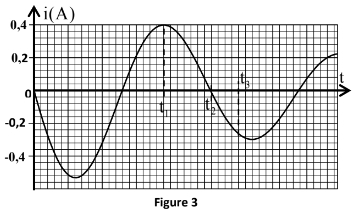
\includegraphics[width=0.5\linewidth]{./img/phys04.png} 

\end{center}

\begin{wrapfigure}[3]{r}{0.25\textwidth}
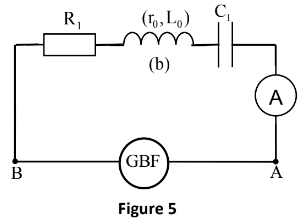
\includegraphics[width=0.9\linewidth]{./img/phys05.png} 
\end{wrapfigure}


\section*{II-Oscillations forcées dans un circuit RLC série (3pts)}
Le circuit représenté sur la figure 5 contient : un générateur, GBF délivrant au circuit une tension sinusoïdale $U_{AB} = 3.\sqrt{2}.cos(2.\pi.N.t)$
Le coefficient de qualité de ce circuit est $Q = 7$, la largeur de la bande passante à $-3dB$ est $14,3Hz$.
A la résonance, l’ampèremètre indique la valeur $I = 1,85.10^2 mA$.

\begin{tblr}{c|[dashed]l}
1  & \textbf{II.1. }Déterminer la fréquence des oscillations électriques à la résonance.\\
1 & \textbf{II.2. }Trouver la valeur de $R_1$ et celle de $C_1$\\
	1 & {\textbf{II.3. }3-3- Calculer la puissance électrique moyenne, consommée par effet joule, dans le circuit \\quand la fréquence prend l’une des valeurs limitant la bande passante.}\\ 

\end{tblr}
\end{document}
